% !TeX spellcheck = en_US
\documentclass[french]{yLectureNote}

\title{Atomistique}
\subtitle{La matière à l'échelle atomique}
\author{Paulhenry Saux}
\date{\today}
\yLanguage{Français}

\professor{J.Cuny}%sebastien.deveuhels.irap.omp.eu

\usepackage{graphicx}%----pour mettre des images
\usepackage[utf8]{inputenc}%---encodage
\usepackage{geometry}%---pour modifier les tailles et mettre a4paper
%\usepackage{awesomebox}%---pour les boites d'exercices, de pbq et de croquis ---d\'esactiv\'e pour les TP de PC
\usepackage{tikz}%---pour deiffner + d\'ependance de chemfig
\usepackage{tkz-tab}
\usepackage{chemfig}%---pour deiffner formules chimiques
\usepackage{chemformula}%---pour les formules chimiques en \'equation : \ch{...}
\usepackage{tabularx}%---pour dimensionner automatiquement les tableaux avec variable X
\usepackage{awesomebox}%---Pour les boites info, danger et autres
\usepackage{menukeys}%---Pour deiffner les touches de Calculatrice
\usepackage{fancyhdr}%---pour les en-t\^ete personnalis\'ees
\usepackage{blindtext}%---pour les liens
\usepackage{hyperref}%---pour les liens (\`a mettre en dernier)
\usepackage{caption}%---pour la francisation de la l\'egende table vers Tableau
\usepackage{pifont}
\usepackage{array}%---pour les tableaux
\usepackage{lipsum}
\usepackage{yFlatTable}
\usepackage{multicol}
\newcommand{\Lim}[1]{\lim\limits_{\substack{#1}}\:}
\renewcommand{\vec}{\overrightarrow}
\begin{document}
\setcounter{chapter}{4}
\chapter{Construire un DOM}
\section{Méthode générale}
On se sert dans cette première partie de la molécule $OH^-$.

On fait le schéma de Lewis de la molécule et on détermine les OA qui sont impliquées dans la liaison.
\begin{enumerate}
 \item On trace un trait vertical pour l'échelle d'énergie
 \item On place les OA selon leur niveau d'énergie. S'il n'est pas précisé, c'est qu'il est sans importance.
\end{enumerate}
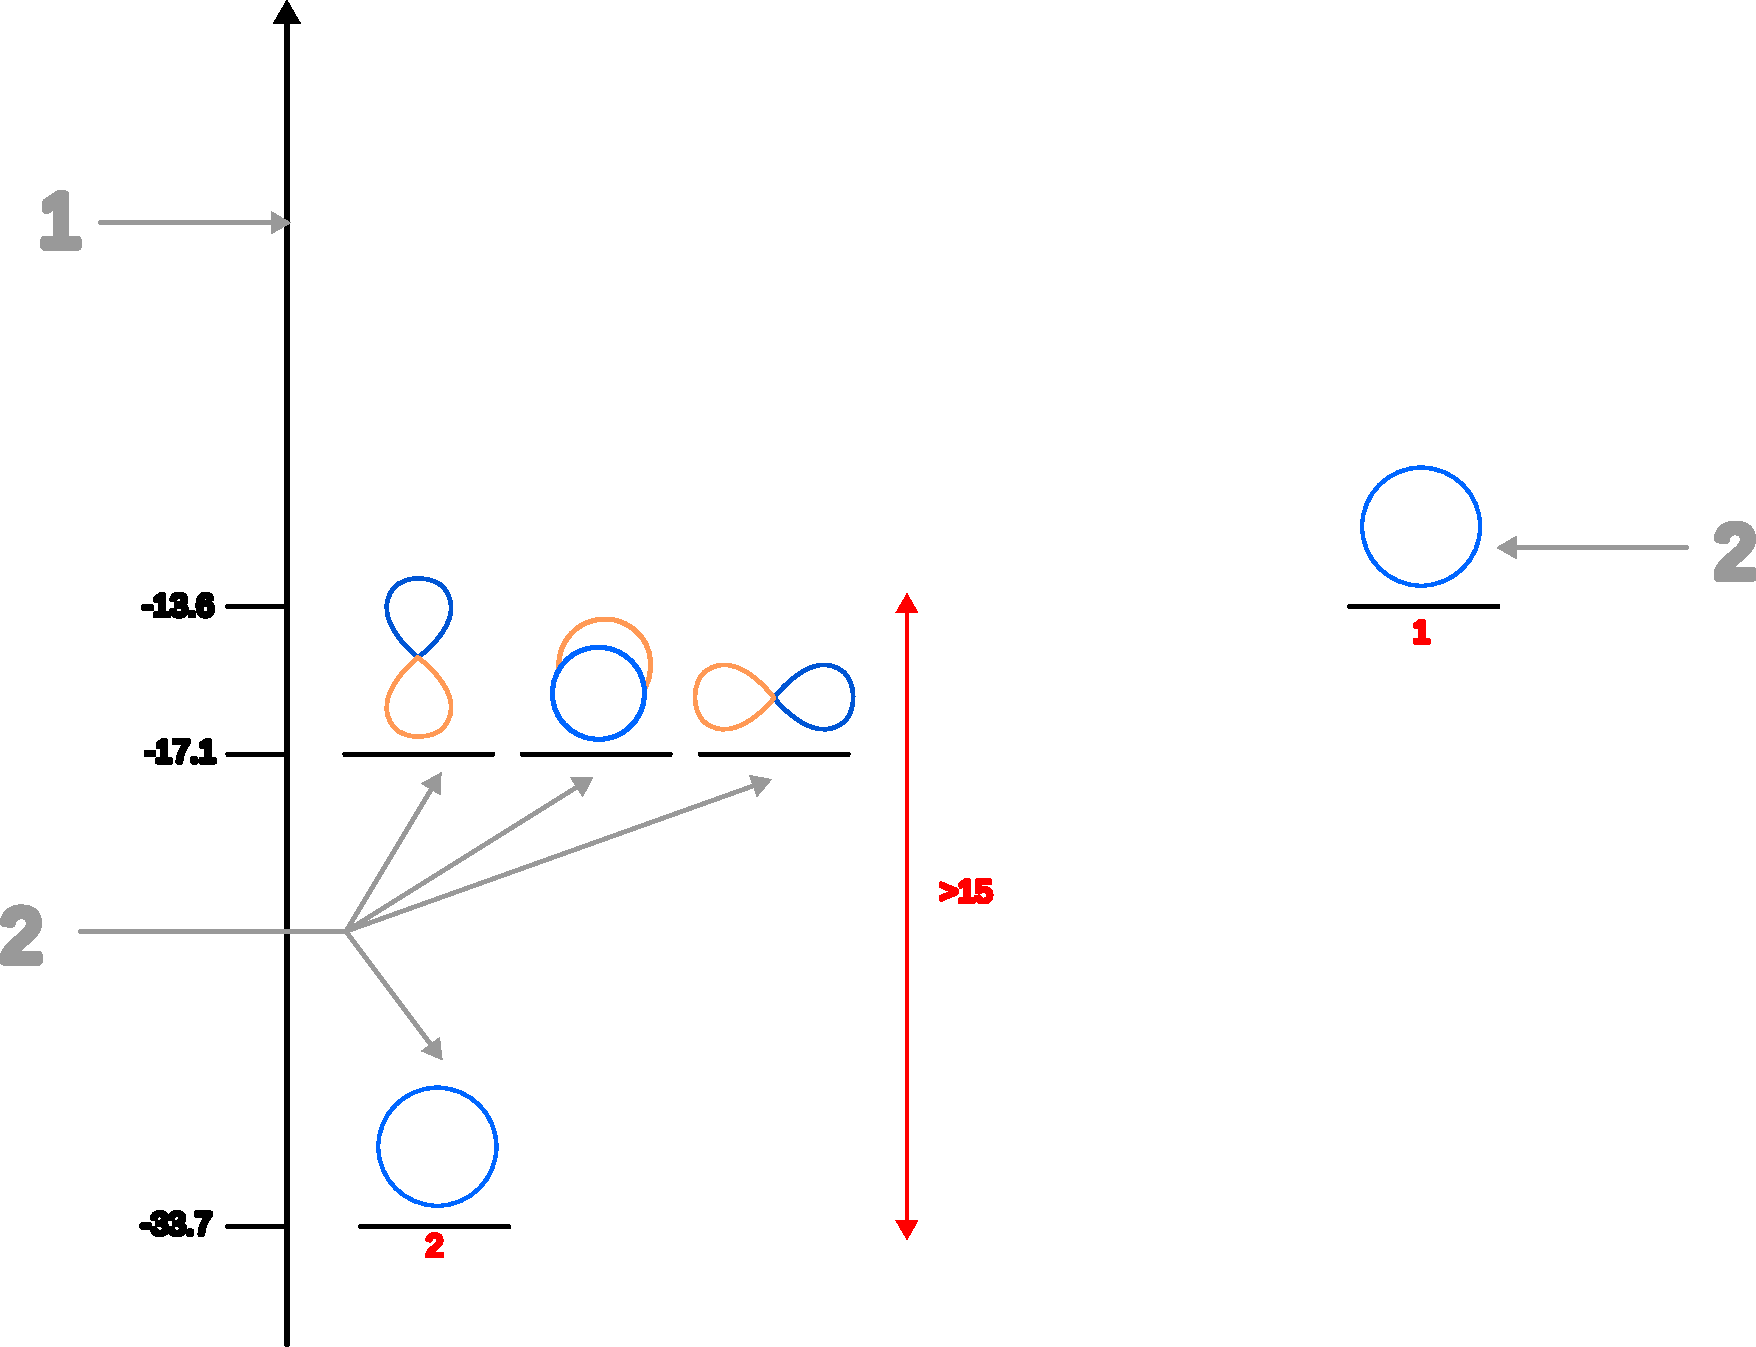
\includegraphics[scale=0.5]{DOM1}
\begin{enumerate}
\setcounter{enumi}{2}
 \item On cherche quelle OA intéragissent. Si les OA sont séparées de plus de 15 eV, on dit que leurs intéractions sont négligeables.
 \item Les OA qui ne réagissent pas restent inchangées, on met juste un trait avec un point pour montrer qu'elles appartiennent à la molécule.
 \item Pour chaque intéraction, on place l'OM liante et l'anti-liante, avec l'anti-liante beaucoup plus haut que la liante est basse. De plus, selon l'énergie des OA formant ces OM, on les dessine avec une taille différente : Plus l'OA est proche du niveau d'énergie de l'OM, plus est dessinée en gros.
 \item Si l'OA est petite par rapport à l'autre, on met la liaison en pointillée
\end{enumerate}
À ce stade, il faut qu'il y ait autant d'OA que d'OM, sinon il y a un problème. C'est aussi la fin des étapes obligatoires. La suite est facultative mais peut servir à donner plus d'informations.

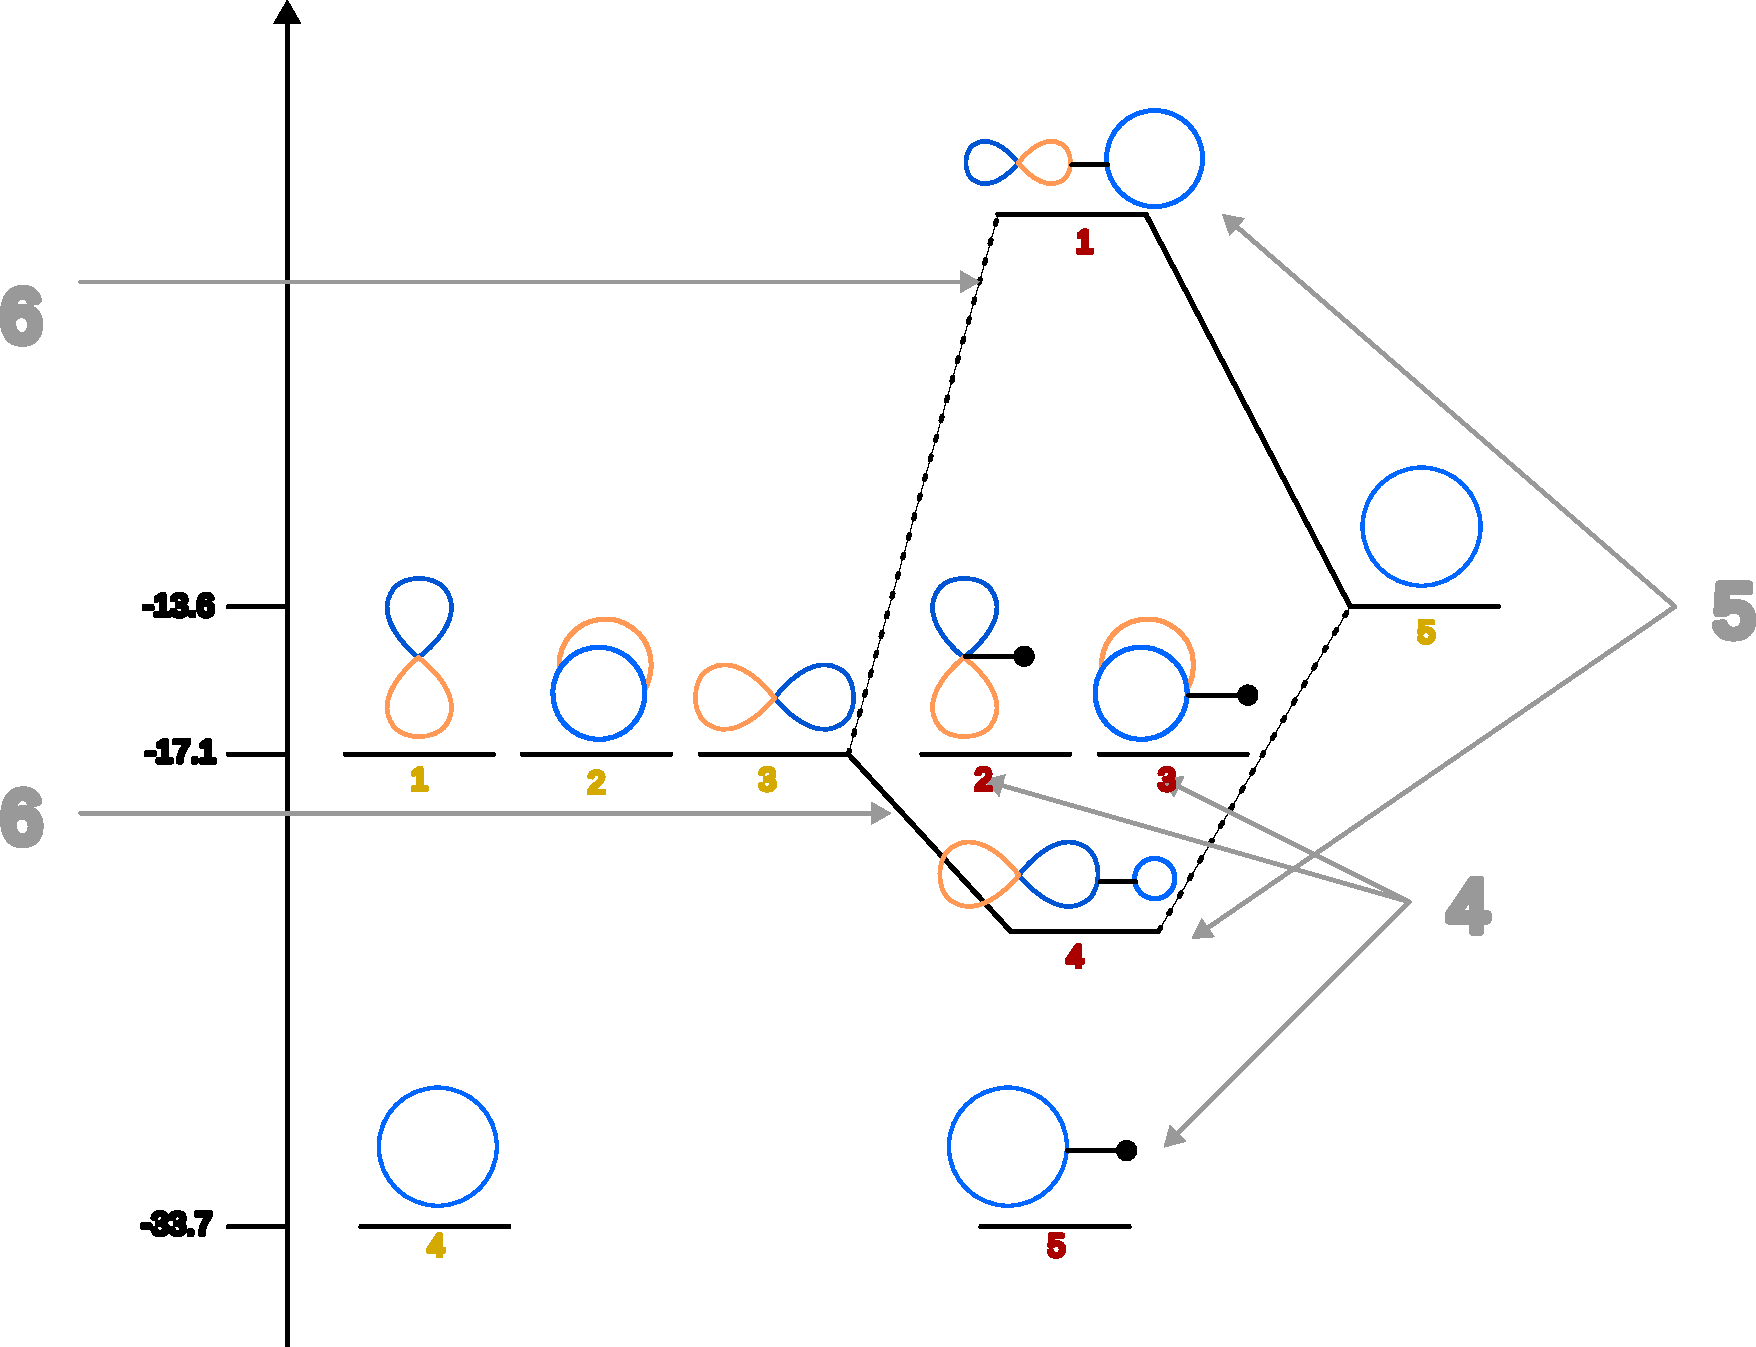
\includegraphics[scale=0.5]{DOM2}
\begin{enumerate}
\setcounter{enumi}{6}
 \item On peut placer les électrons, en suivant les m\^eme règles que pour le placement des électrons dans les OA.
 \item On peut donner le type de liaison. Les OM liantes sont notée $\sigma$, les anti-liantes $\sigma *$ et les non-liantes $\pi$
\end{enumerate}
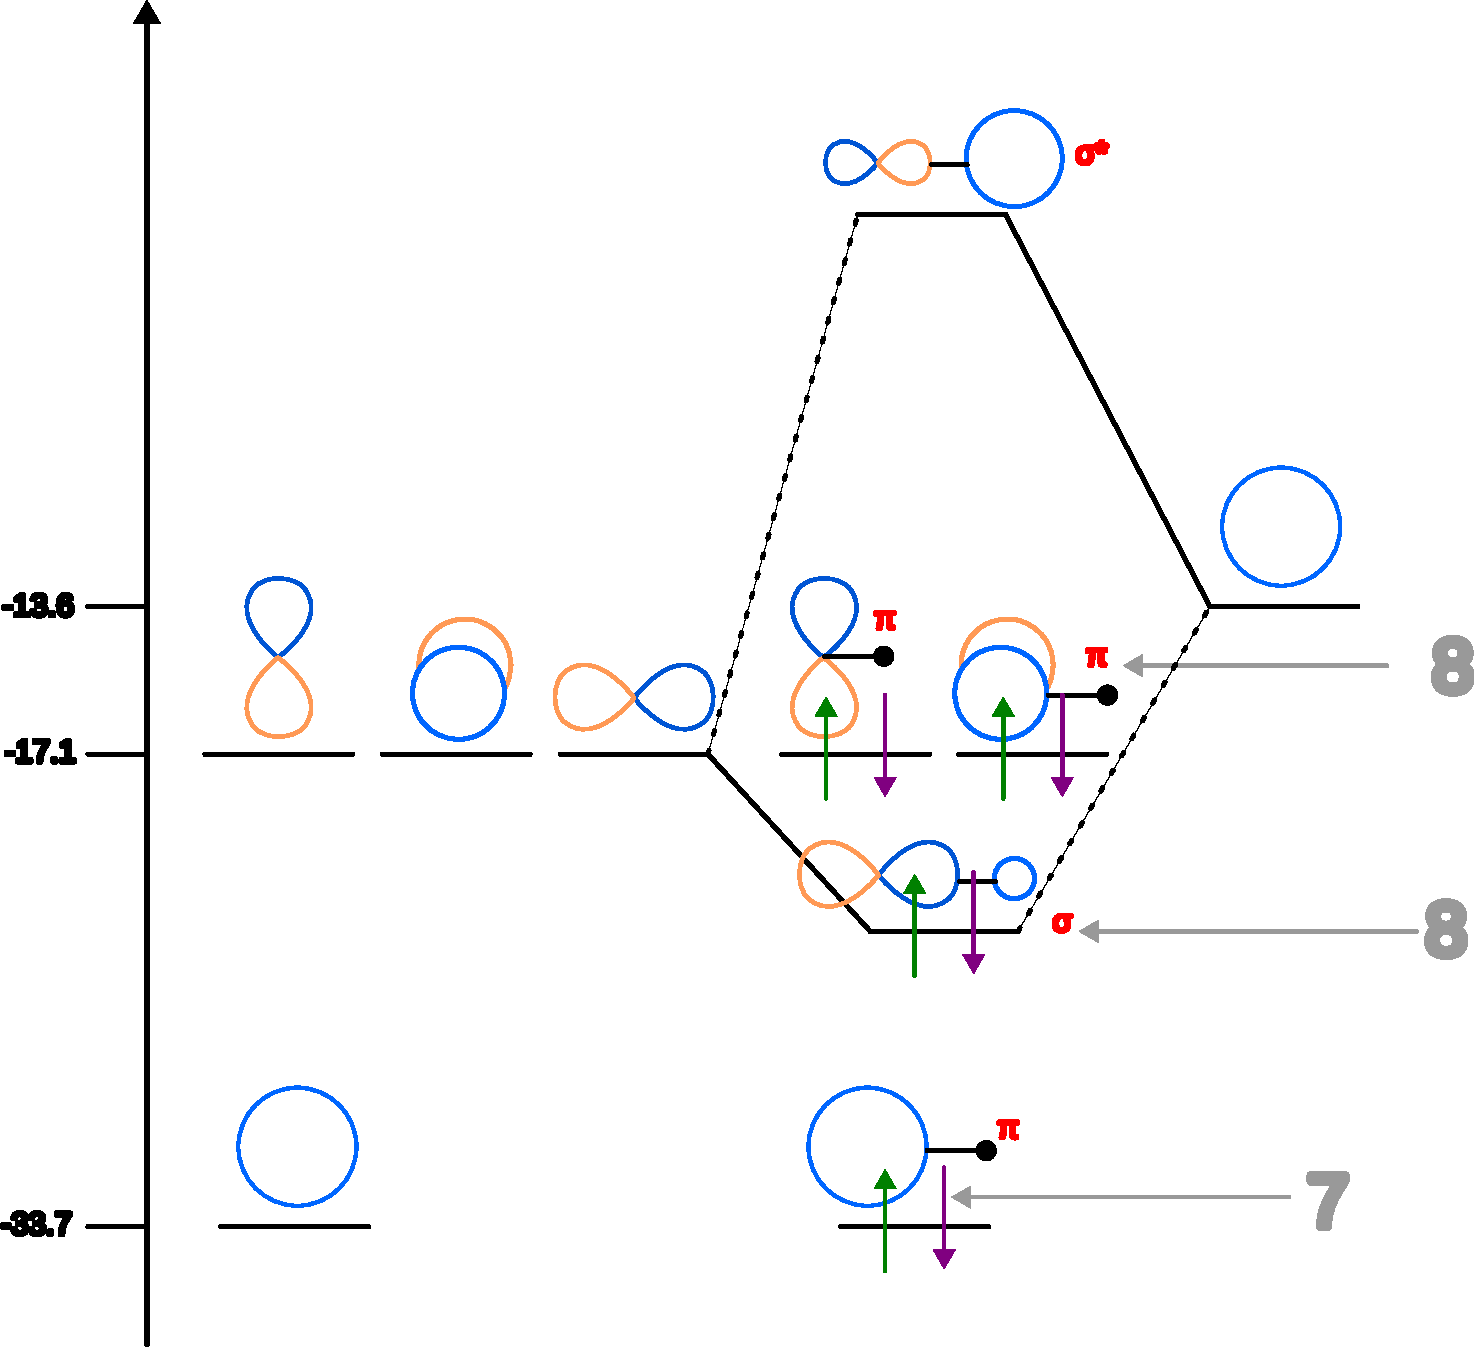
\includegraphics[scale=0.5]{DOM3}
\section{Cas particuliers}
Pour ces deux dernières étapes, on prend la molécule $O_2$
\begin{enumerate}
\setcounter{enumi}{8}
\item On indique si les liaisons des OM sont $\pi$ ou $\sigma$. On met un numéro pour différencier les systèmes d'OM et indiquer quelle OM liante correspond à quelle OM non Anti-liante.
 \item Pour des molécules possédants un centre d'inversion, on indique sur les OM si elles sont symétriques par rapport à leur centre d'inversion ou anti-symétriques (symétriques en changeant de signe). Dans le premier cas, on les annote avec un $g$, ``gegen'', symétrique en allemand et dans le second cas avec un $u$, ``ungegen'', anti-symétrique.
\end{enumerate}
On remarque que les OM 1 ont plus d'énergie que l'OM 2 car elles se recouvrent moins que l'OM 2, dont les lobes sont dans le m\^eme axe. C'est pourquoi, on les place au-dessus de l'OM 2.

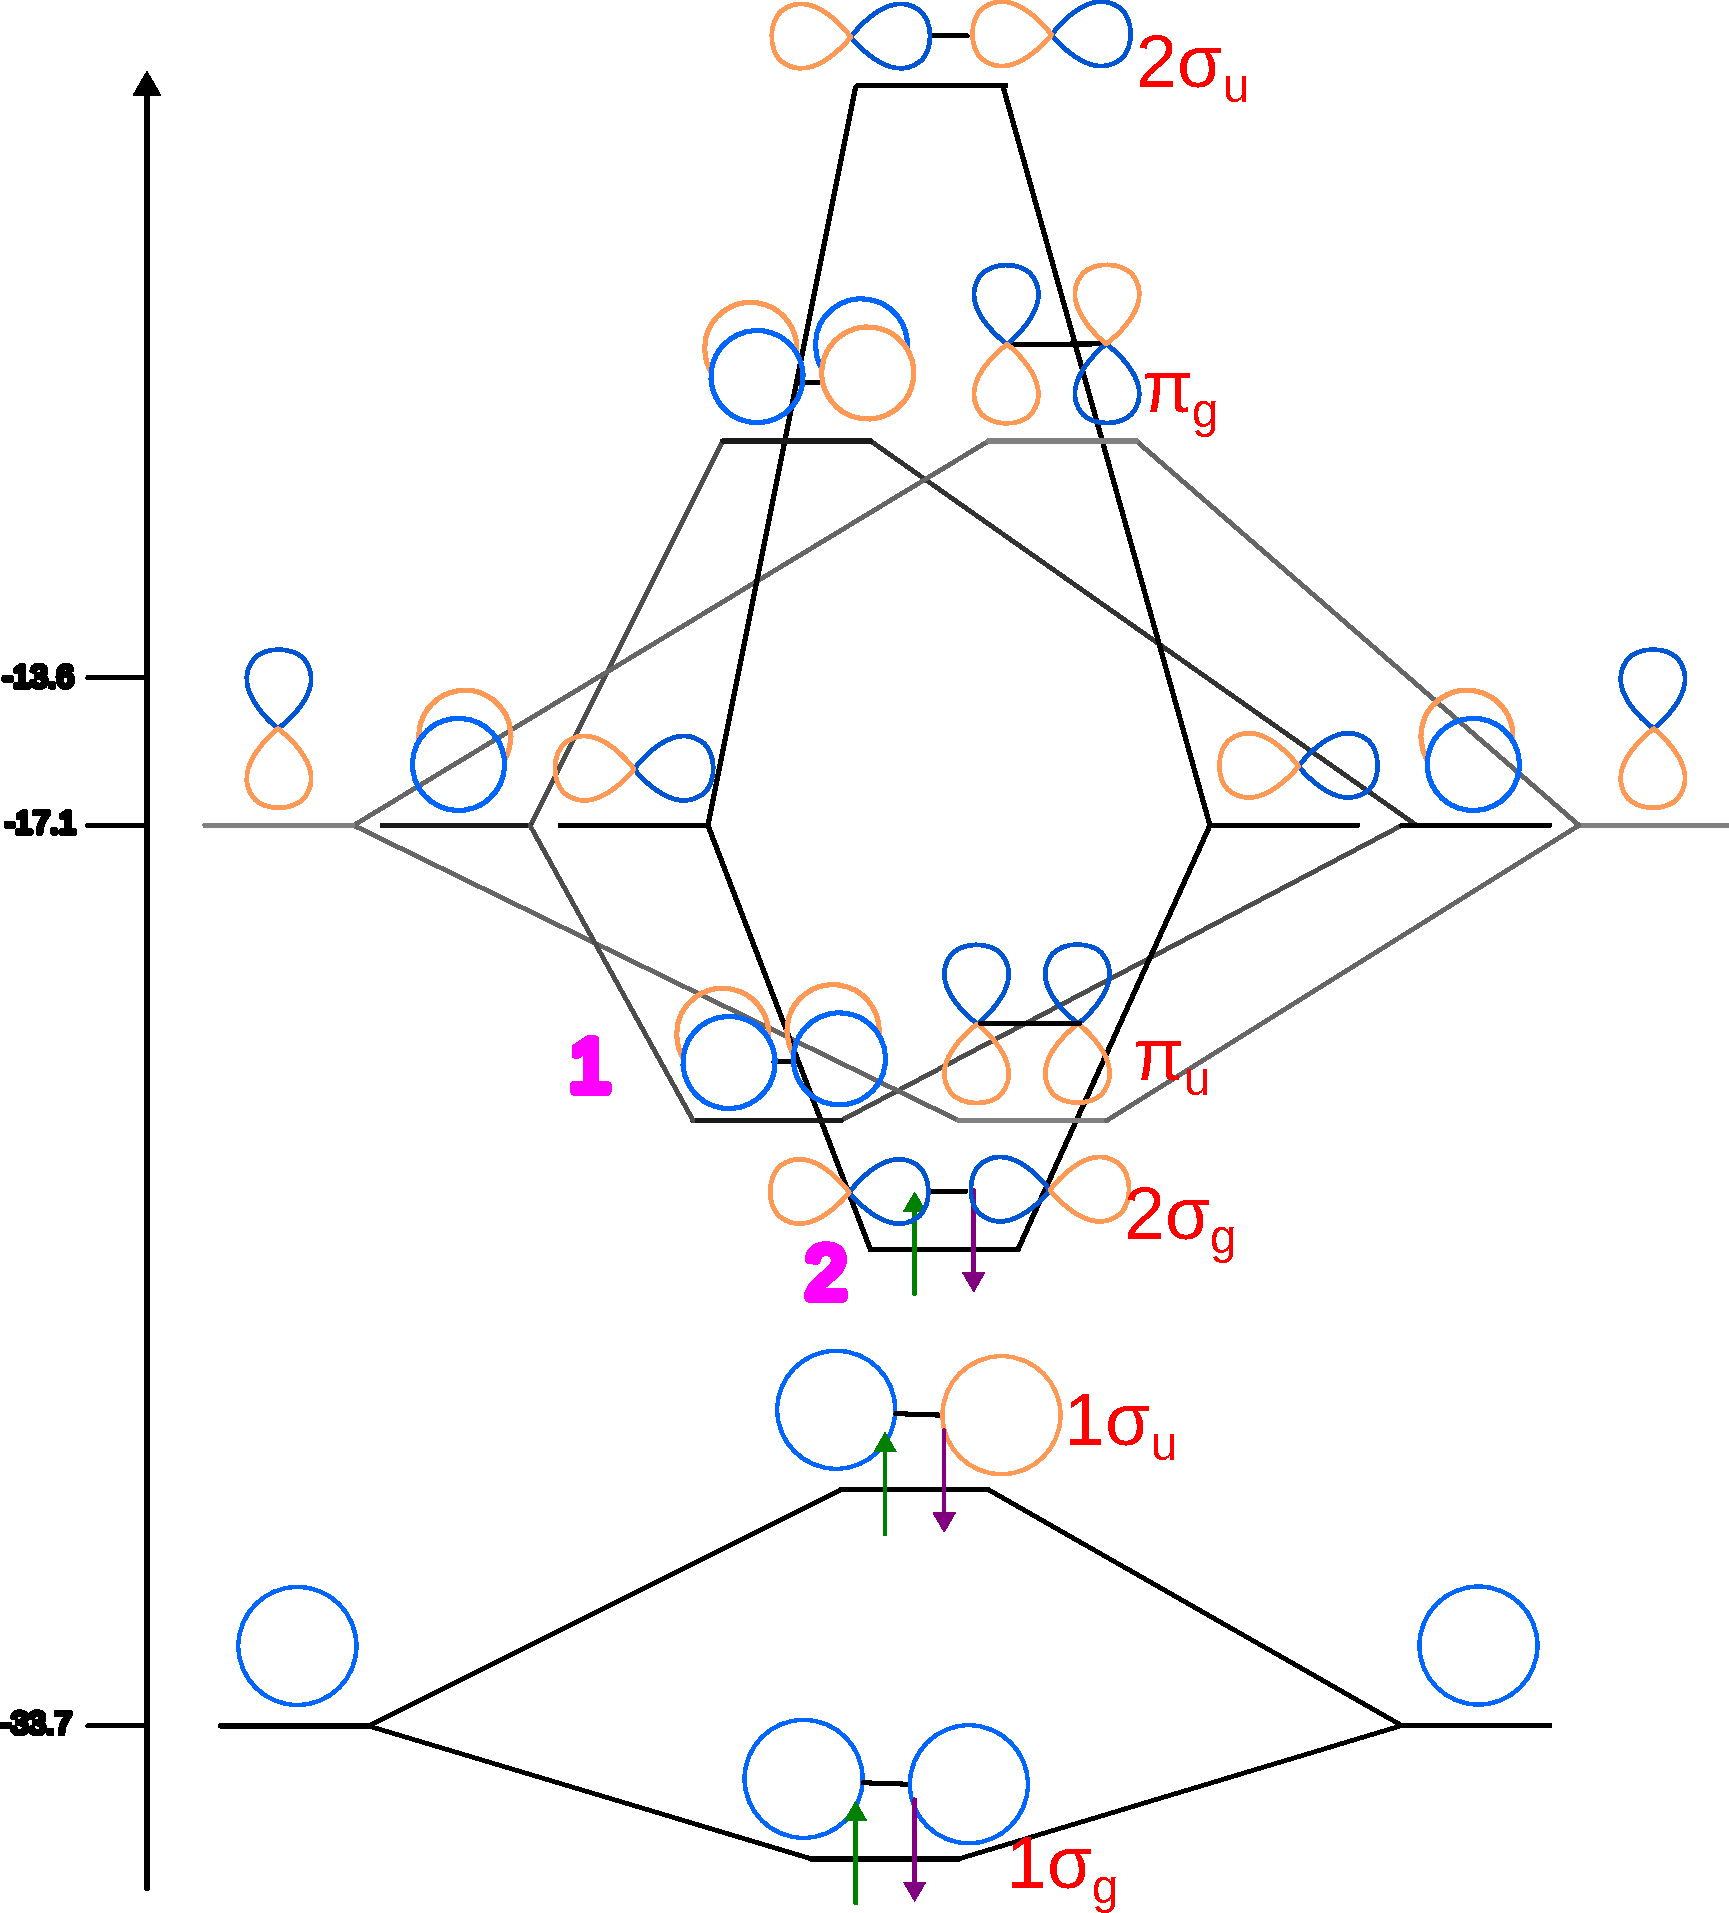
\includegraphics[scale=0.5]{DOM4}

\end{document}

